\documentclass{article}
\usepackage[utf8]{inputenc}
\title{Video 1: Why Sums And Averages Tend To Look Gaussian}
\author{wbg231 }
\date{December 2022}
\newcommand{\R}{$\mathbb{R}$}
\newcommand{\B}{$\beta$}
\newcommand{\A}{$\alpha$}
\newcommand{\D}{\Delta}

\newcommand{\avector}[2]{(#1_2,\ldots,#1_{#2})}
\newcommand{\makedef}[2]{$\textbf{#1}$:#2 }
\usepackage{tikz,graphicx,hyperref,amsmath,amsfonts,amscd,amssymb,bm,cite,epsfig,epsf,url}

\begin{document}

\maketitle

\section{introduction}
\begin{itemize}
\item \href{https://www.youtube.com/watch?v=-fBN9z6uc_E&list=PLBEf5mJtE6KuZ5NBQMuWIMsiOOrV9ibzm&index=70}{video link}
\section{sum of discreet rv}
\subsection{soccer league example}
\item points $\Tilde{x}_i$ in game i. gamer are independent 
\item $P(\Tilde{x}_i=0)=.3$ $P(\Tilde{x}_i=1)=.3$ $P(\Tilde{x}_i=2)=.3$
\item we want to characterize the distribution $\Tilde{s}_{n}=\Sigma_{i=1}^{n}\Tilde{x}_i$
\item lets think about the distribution of the sum of points over just two games
\begin{itemize}
    \item  so they can either earn 0, 1, 2, 3, 4, 6 points
    \item $P(\Tilde{s}=0)=P(\Tilde{x}_1+\Tilde{x}_2=0)P(\Tilde{x}_1=0,\Tilde{x}_2=0)=P(\Tilde{x}_1=0)P(\Tilde{x}_2=0)=.09$
    \item $P(\Tilde{s}=1)=P(\Tilde{x}_{1}+\Tilde{x}_{2}=1)=P(\Tilde{x}_1=0, \Tilde{x}_2=1)+P(\Tilde{x}_1=1, \Tilde{x}_2=0)=(.3)(.3)+.3(.3)=.09+.09=.18$
    \item 
\end{itemize}
\subsection{sum of two independent discrete random variables}
\item consider random variable $\Tilde{a}$ with range A, $\Tilde{b}$ with rang B
\item the pmf of $\Tilde{s}=\Tilde{a}+\Tilde{b}$ is 
\item $P(\Tilde{s}=s)=P(\Tilde{a}+\Tilde{b}=s)=\Sigma_{a\in A}P(\Tilde{a}=a,\Tilde{b}=s-a)=\Sigma_{a\in A}P(\Tilde{a}=a)P(\Tilde{b}=s-a)=\Sigma_{i=-\infty}^{\infty}P(\Tilde{a}=a)P(\Tilde{b}=s-a)$
\item this last term $\Sigma_{i=-\infty}^{\infty}P(\Tilde{a}=a)P(\Tilde{b}=s-a)$ is the convolution of the pmf of a on b, such that $\Sigma_{i=-\infty}^{\infty}P(\Tilde{a}=a)P(\Tilde{b}=s-a)=P_{\Tilde{a}}*p_{\Tilde{b}}(s)$ the convolution is an operation where for a fixed value of s, we take a function, and overlay with with a shifted function and take the sum 
\subsection{sum of n independint random vairbles}
\item for discrete independint rvs $\Tilde{a}_1..\Tilde{a}_{n}$ with inter values 
\item the pmf there sum $\Tilde{s}=\Sigma_{i=1}^{n}\Tilde{a}_{i}$ is $$P_{\Tilde{s}}(s)=P(\Tilde{s}=s)=P(\Sigma_{i=1}^{n}\Tilde{a}_i=s=P(\Sigma_{a \in A_1} a\Sigma_{i=2}^{n}\Tilde{a}_i=p_{\Tilde{a}_1}* \Sigma_{i=2}^{n}\Tilde{a}=p_{\Tilde{a}_1}*p_{\Tilde{a}_2}...*p_{\Tilde{a}_n}(s)$$
\subsection{graphical result for sum of soccer gamer}
\item 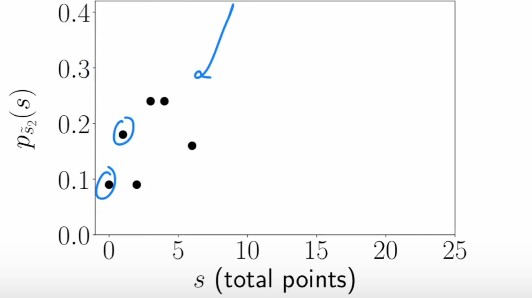
\includegraphics[width=10cm]{notes/week_4/vidio 1: Why Sums And Averages Tend To Look Gaussian/immages/v1_1.jpg}
\item here is the pmf for $\Tilde{s}_{2}$ ie the sum of points over two soccer games 
\item by our result above $\Tilde{s}_{3}=\Tilde{s}_{2}*\Tilde{s}_{1}(S)$ so in other words every added game is making the result of the sum more into a weighted sum  (ie convolution) over all possible outcomes. this has a smooth effect an over time we get something like this which is smooth and looks Gaussian 
\item here is the distribution of $\Tilde{s}_{8}\\$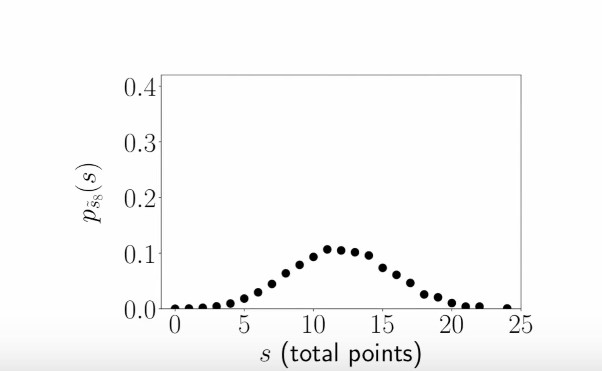
\includegraphics[width=10cm]{notes/week_4/vidio 1: Why Sums And Averages Tend To Look Gaussian/immages/v1_2.jpg}

\subsection{Gaussian approximation }
\item lets try to approximate this distribution using a Gaussian rv with the same mean and variance 
\item what is $E{\Tilde{s}_[n]}=E[\Sigma_{ii=1}^{n}x_i]=\Sigma_{i=1}^{n}E[\Tilde{x}_i]=1.5(n)$
\item what about the variance? $var(\Tilde{s}_{n})=var(\Tilde{S}_{n})=\Sigma_{i=1}^{n}var(\Tilde{x}_i)=1.65n$ \textbf{this variance result requires that the random variables are independent} 
\item so here is what overlaying a Gaussian with this mean and variance with our soccer example looks like 
\item for two games it is not great \\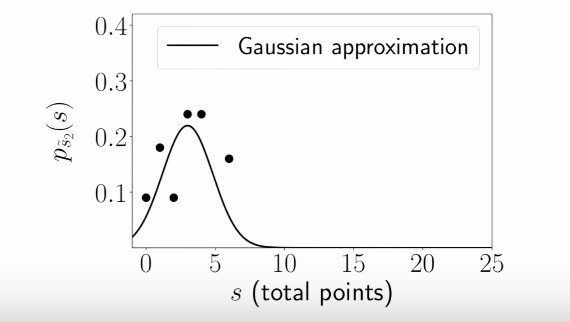
\includegraphics[width=10cm]{notes/week_4/vidio 1: Why Sums And Averages Tend To Look Gaussian/immages/v1_3.jpg}
\item for 9 games it is very close \\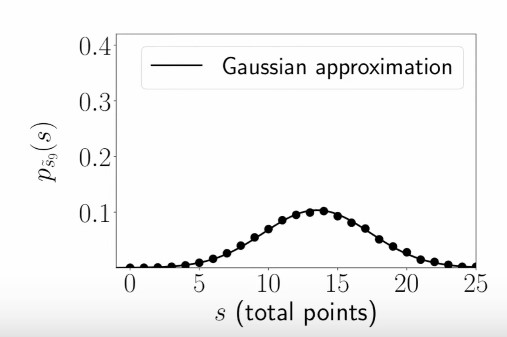
\includegraphics[width=10cm]{notes/week_4/vidio 1: Why Sums And Averages Tend To Look Gaussian/immages/v1_4.jpg}
\item so we can see that this works fairly well even with a relatively small n ,and this is why we will later on use the central limit theorem to model sums of independent rv, even with a limited number of n 
\section{sum of continuous rv}
\subsection{coffee supply example}
\item suppose there is a cafe that is worries about coffee supply 
\item they have n independent suppliers, that can supply an uncertain amount of Coffey
\item for each supplier the amount of coffee they can supply is uniform between 0,1 
\item the total amiable coffee $\Tilde{s}_{n}=\Sigma_{i=1}^{n}\Tilde{c}_{i}$
\item so to avoid risk they just buy $\Tilde{m}_{n}=\frac{\Tilde{s}_{n}}{n}$ so they are distributing the risk over all suppliers 
\subsection{two suppliers}
\item so $F(\Tilde{s}_{2}\leq s)=P(\Tilde{c}_{1}+\Tilde{c}_2\leq s)=\int_{c_{1}=-\infty}^{\infty}\int_{c_2=-\infty}^{s-c1}f_{\Tilde{c}_1}(c_1)f_{\Tilde{c}_2}(c_2)dc_{1}dc_{2}=\int_{c_{1}=-\infty}^{\infty}f_{\Tilde{c}_{1}}(c_1)F_{\Tilde{c}_2}(s-c_1)dc_1$
\item now to find the pdf we need to take the derivative of this quantity so $f_{\Tilde{s}_2}(s)=\frac{d}{ds}F_{\Tilde{s}_2}(s)=\frac{d}{ds}\int_{c_{1}=-\infty}^{\infty}f_{\Tilde{c}_{1}}(c_1)F_{\Tilde{c}_2}(s-c_1)dc_1=\int_{c_{1}=-\infty}^{\infty}f_{\Tilde{c}_{1}}(c_1)f_{\Tilde{c}_2}(s-c_1)dc_1$
\item so we know $f_{\Tilde{s}_2}(s)=\int_{c_{1}=-\infty}^{\infty}f_{\Tilde{c}_{1}}(c_1)f_{\Tilde{c}_2}(s-c_1)dc_1$
\item further we know that both $\Tilde{c}_{1}, \Tilde{c}_{2}$ are uniform between zero and 1. 
\item thus it must be the case that $f_{\Tilde{c}_{1}}(a)=1$ if $a\in [0,1]$
\item$\Tilde{c}_{2}(s-a)=1$ if $0\leq s-a\leq 1\Rightarrow s\leq -a\leq 1+s\Rightarrow s-1\leq a\leq s$
\item so at any given point of s the value of our integral is the green area in this picture because it is the area where neither $c_1$ nor $c_2$ are zero \\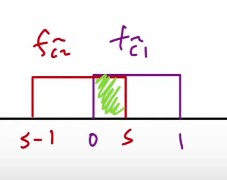
\includegraphics[width=10]{notes/week_4/vidio 1: Why Sums And Averages Tend To Look Gaussian/immages/v1_5.jpg}
\item then we drag our value s over all possible values creating kind of a smoothed withed sum of the Pd's, and when they stop overlapping we get zero. 
\item so we are kind of smoothing out one pdf by doing a weighted average with the other pdf
\item so if $s\in [0,1]$ then $f_{\Tilde{s}_2}(s)=\int_{c_{1}=-\infty}^{\infty}f_{\Tilde{c}_{1}}(c_1)f_{\Tilde{c}_2}(s-c_1)dc_1=\int_{a=0}^{s}f_{\Tilde{c}_{1}}(a)f_{\Tilde{c}_2}(s-a)da=\int_{a=0}^{s}1*1da=s$
\item so if $s\in [1,2]$ then $f_{\Tilde{s}_2}(s)=\int_{c_{1}=-\infty}^{\infty}f_{\Tilde{c}_{1}}(c_1)f_{\Tilde{c}_2}(s-c_1)dc_1=\int_{a=s-1}^{1}f_{\Tilde{c}_{1}}(a)f_{\Tilde{c}_2}(s-a)da=\int_{a=s-1}^{1}1*1da=1(1-s+1)=2-s$
\item if $s<0 \text{ or } s>2$ then $f_{\Tilde{s}_2}(s)=\int_{c_{1}=-\infty}^{\infty}f_{\Tilde{c}_{1}}(c_1)f_{\Tilde{c}_2}(s-c_1)dc_1=0$
\subsection{purchase coffee}
\item so recall that $\Tilde{m}_{n}=\frac{\Tilde{s}_{n}}{n}$
\item so what is $F_{\Tilde{m}_{2}}(m)=P(\Tilde{m}_{2}\leq m)=P(\frac{\Tilde{s}_{n}}{n}\leq m)=P(\Tilde{s}_{n}\leq nm)=F_{\Tilde{s}_{n}}(2m)$
\item then differentiating we can see that $f_{\Tilde{m}_{2}}(m)=\frac{d}{dm}F_{\Tilde{s}_n}(2m)=2\frac{d}{ds}F_{\Tilde{s}_n}(2m)=2f_{\Tilde{s}_{n}}(2m)$
\item then we can see that $f_{\Tilde{m}_{n}(m)}=f_{\Tilde{s}_{n}(nm)}=4m$ if $s\in [0,\frac{1}{2}]$
\item then we can see that $f_{\Tilde{m}_{n}(m)}=f_{\Tilde{s}_{n}(nm)}=4(1-m)$ if $s\in [\frac{1}{2},1]$
\item then we can see that $f_{\Tilde{m}_{n}(m)}=f_{\Tilde{s}_{n}(nm)}=0$ otherwise
\item so the pdf of the purchased coffee from one supplier will look uniform \\ 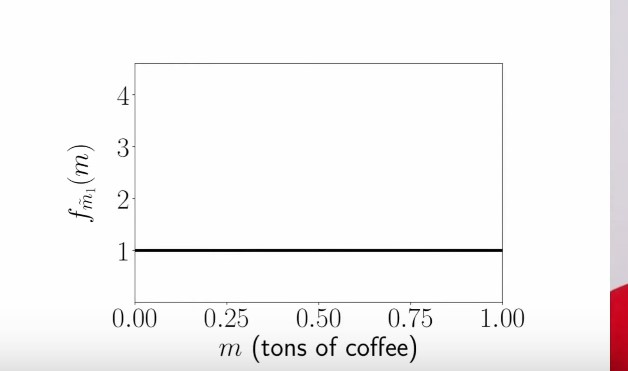
\includegraphics[width=10cm]{notes/week_4/vidio 1: Why Sums And Averages Tend To Look Gaussian/immages/v1_6.jpg}
\item then for two suppliers we know that we are going to be involving the pdf of the suppliers that is $\Tilde{m}_{2}=\frac{1}{2}\Tilde{s_2}=\frac{1}{2}(f_{\Tilde{c}_{1}}*f_{\Tilde{c}_2}(s))$
\item so the pdf of two suppliers looks like 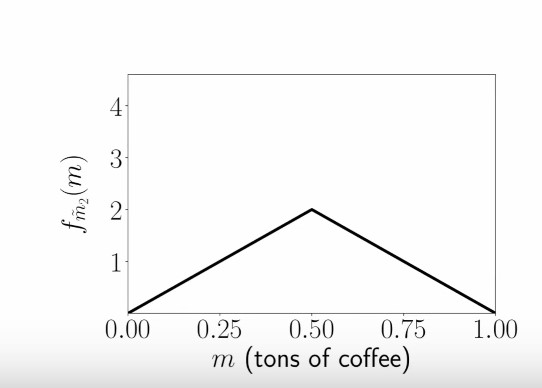
\includegraphics[width=10cm]{notes/week_4/vidio 1: Why Sums And Averages Tend To Look Gaussian/immages/v1_7.jpg}
\item so think of this shape as coming from the convolution operation where we are taking a weighted average of all the possible outcomes. so the likelihood of the sum of both suppliers having s is the likelihood of $c_1$ having all possible values times the likelihood of the $c_2$ having the value s-a. thus. we get this triangle shape as values from the center of the distribution become less likely 
\item so when we have n suppliers $f_{\Tilde{s}_{n}}(s)=f_{\Tilde{c}_1}*f_{\Tilde{c}_2}...f_{\Tilde{c}_n}$ so then we can see that $f_{\Tilde{m}_{n}}(m)=nf_{\Tilde{s}_{n}}(nm)=n(f_{\Tilde{c}_1}*f_{\Tilde{c}_2}...f_{\Tilde{c}_n}(nm)$
\item 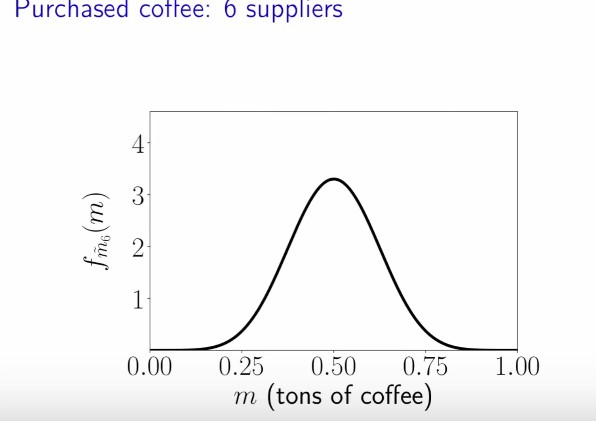
\includegraphics[width=10cm]{notes/week_4/vidio 1: Why Sums And Averages Tend To Look Gaussian/immages/v1_8.jpg}
\item so over time this ends up looking quite Gaussian 
\item so look that the convolution smooth out the pdf, and these things look very closely Gaussian. 

\subsection{sum of independent continuous rv}
\item given continuous rvs $\Tilde{a}$, $\Tilde{b}$ the pdf of $\Tilde{s}=\Tilde{a}+\Tilde{b}$ is 
\item $f_{\Tilde{s}}(s)=\int_{a=-\infty}^{\infty}f_{\Tilde{a}}(a)f_{\Tilde{b}}(s-a)da=f_{\Tilde{a}}*f_{\Tilde{b}}(s)$ so this is a continuous convolution 
\subsection{sum of Gaussian}
\subsection{independent standard Gaussian a and b}
\item suppose we have to independent standard Gaussian rv $\Tilde{a}, \Tilde{b}$
what is the pdf of there sum $\Tilde{s}=\Tilde{a}+\Tilde{b}$
\item $f_{\Tilde{s}}(s)=\int_{a=-\infty}^{\infty}f_{a}(a)f_{b}(s-a)da=\int_{a=-\infty}^{\infty}\frac{1}{2\pi}e^{-\frac{a^2}{2}}\frac{1}{2\pi}e^{-\frac{(s-a)^2}{2}}da=\int_{a=-\infty}^{\infty}\frac{1}{2\pi}e^{-\frac{1}{2} (a^2+(s-a)^2)}da=\int_{a=-\infty}^{\infty}\frac{1}{2\pi}e^{-a^2-as+\frac{s^2}{2})}da=\int_{a=-\infty}^{\infty}\frac{1}{2\pi}e^{-(a-\frac{s}{2})^2-\frac{s^2}{4})}da$
\item then we can separate this as the product of two Gaussian like this $f_{\Tilde{s}}(s)=\int_{a=-\infty}^{\infty}\frac{1}{2\pi}e^{-(a-\frac{s}{2})^2-\frac{s^2}{4})}da=\frac{1}{\sqrt{2\pi}\sigma}e^{-\frac{s^2}{2\sigma^2}}\int_{a=-\infty}^{\infty}\frac{1}{\sqrt{2\pi}\sigma^{-1}}e^{-\frac{(a-\frac{s}{2})^2}{s\sigma^{-2}}}da$ where $\simga^{2}=2$
\item notice further that this $\int_{a=-\infty}^{\infty}\frac{1}{\sqrt{2\pi}\sigma^{-1}}e^{-\frac{(a-\frac{s}{2})^2}{s\sigma^{-2}}}da$ is the integral of a pdf over the real numbers and thus equals 1. 
\item thus we have $f_{\Tilde{s}}(s)=\frac{1}{\sqrt{2\pi}\sigma}e^{-\frac{s^2}{2\sigma^2}}\int_{a=-\infty}^{\infty}\frac{1}{\sqrt{2\pi}\sigma^{-1}}e^{-\frac{(a-\frac{s}{2})^2}{s\sigma^{-2}}}da=\frac{1}{\sqrt{2\pi}\sigma}e^{-\frac{s^2}{2\sigma^2}}$ so this is a pdf with zero mean and variance equal to 2. 
\item so the convolution of two Gaussian's remains Gaussian 
\item and this makes sense since when we convovle other random variables they look Gaussian 
\subsection{independent general Gaussian rv}
\item you can follow the same argument to show that if $\Tilde{a}_1,\Tilde{a}_2$ are Gaussian with means $\mu_1,\mu_2$ and variances $\simga_{1}^{2},\simga_{2}^{2}$
\item the sum $\Tilde{s}=\Tilde{a}_1+\Tilde{a}_2$ will be Gaussian with mean $\mu_1+\mu_2$ and variance $\simga_1+\simga_2$ 
\end{itemize}
\end{document}
